\documentclass[letterpaper]{article} 
\usepackage{graphicx}
\usepackage{caption}
\usepackage{subcaption}
\usepackage[margin=.5in]{geometry}

\renewcommand{\thefigure}{R\arabic{figure}} % figure numbering for rebuttal only

\DeclareGraphicsExtensions{.pdf,.png,.jpg,.mps,.eps,.ps}
\graphicspath{{../../figures/inv_man/}}

\begin{document}

\begin{figure}[tbhp]
  \centering
  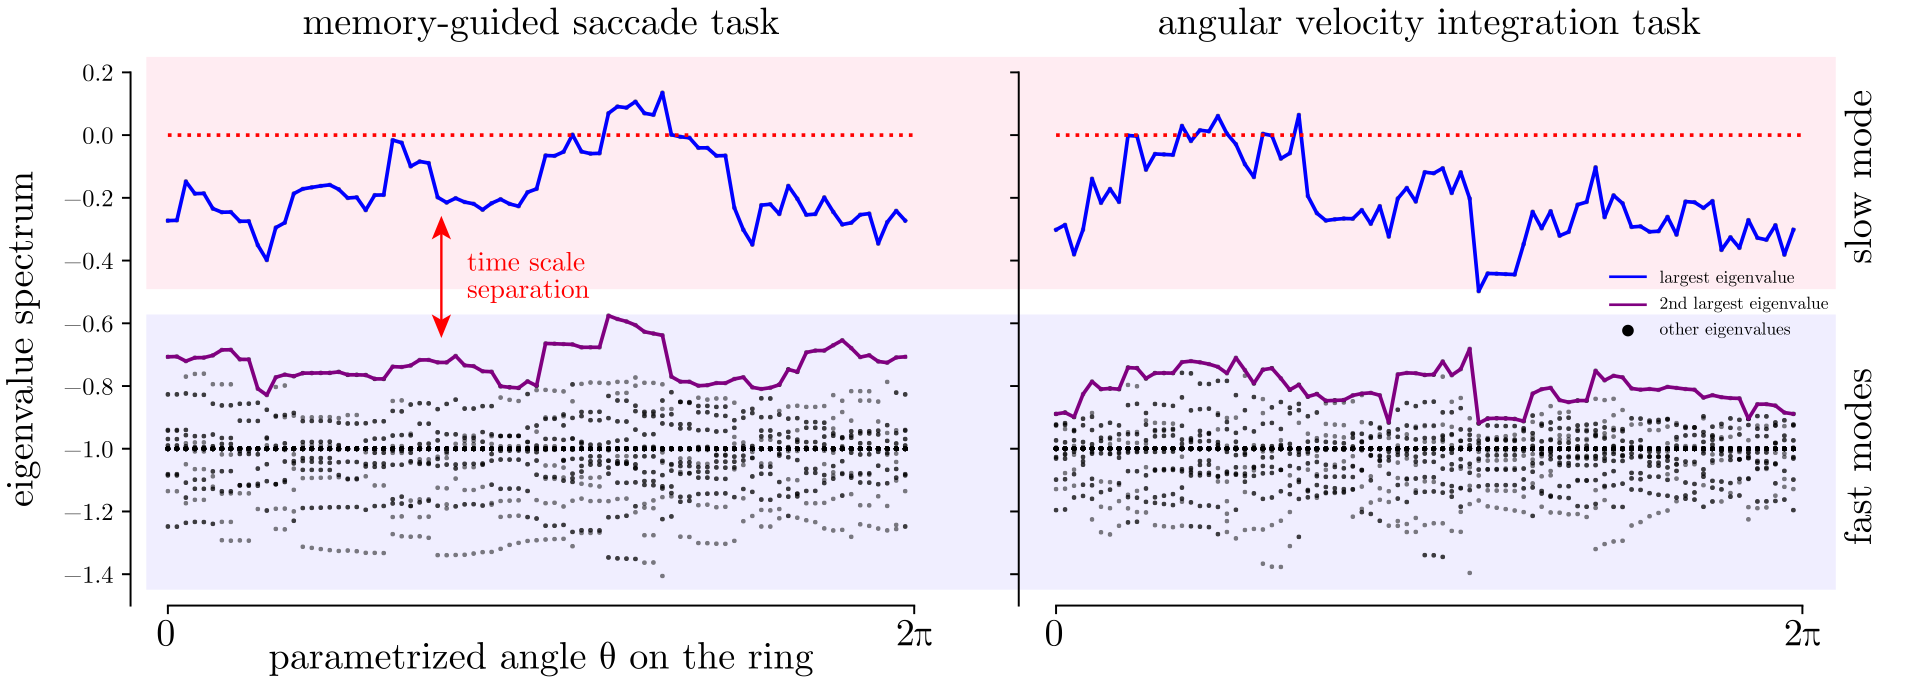
\includegraphics[width=0.8\textwidth]{eigenvalue_gap}
  \caption{The eigenvalue spectrum for  trained networks  show a gap between the first two largest eigenvalues.
    \textbf{(A)} Example network trained on the memory-guided saccade task (Fig.4B in the main text).
    \textbf{(B)}  Example network trained on the angular velocity integration task (Fig.4C in the main text).
}\label{fig:eigenvalue_gap}
\end{figure}


\begin{figure}[tbhp]
  \centering
  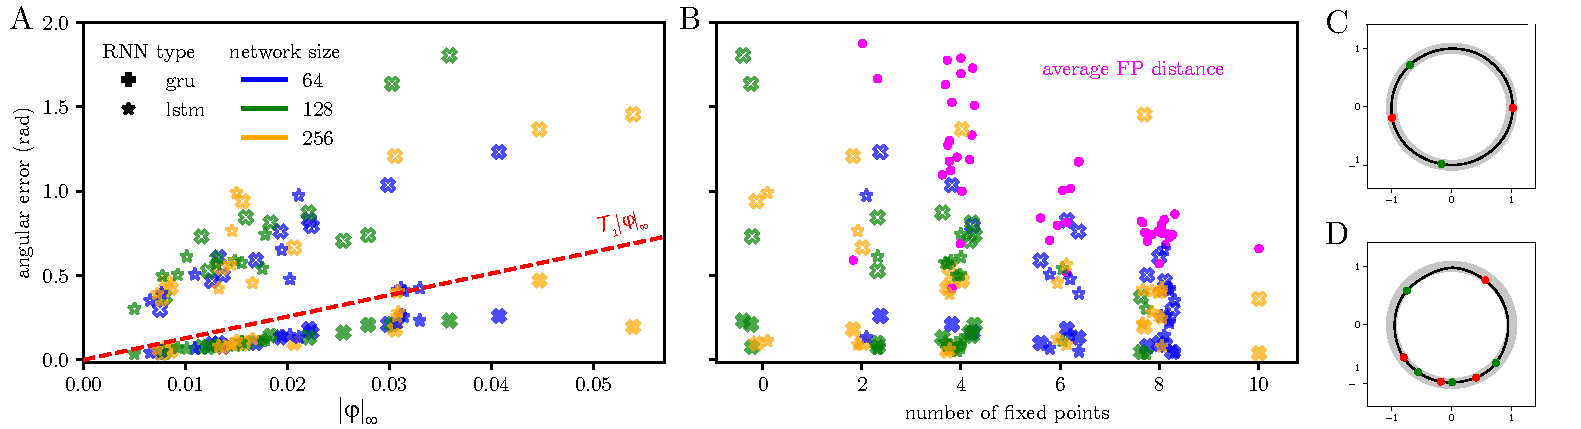
\includegraphics[width=\textwidth]{angular_losses_lstm_gru}
  \caption{The different measures for memory capacity reflect the generalization properties implied by the topology of the found solution.
    \textbf{(A)} The average accumulated angular error versus the uniform norm on the vector field shown.
     Time of trial length on which networks were trained, \(T_1\)) indicated with filled markers and at asymptotic time (with hollow markers).
      The number of fixed point is an integer number. The points are spread out slightly to aid visibility.
    \textbf{(B)}  The number of fixed points versus average accumulated angular error, with the average distance between neighbouring fixed points indicated in magenta.
}\label{fig:angular_losses_lstm_gru}
\end{figure}
%A==A
%B==C in main text


\begin{figure}[tbhp]
  \centering
  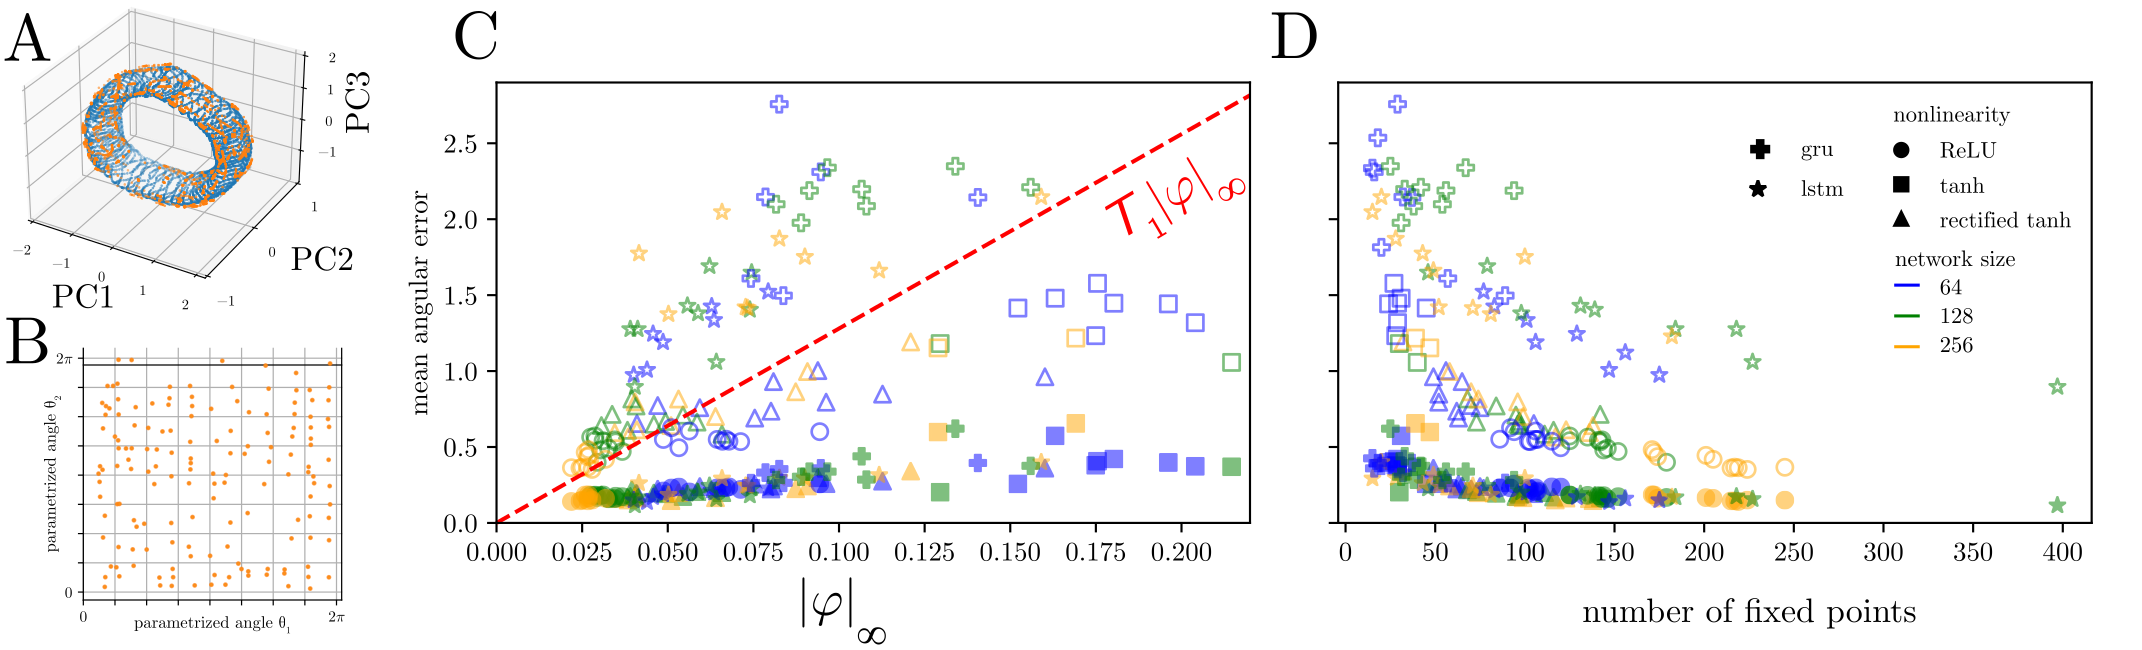
\includegraphics[width=\textwidth]{davit}
  \caption{Networks trained on a double angular velocity integration task.
    \textbf{(A)} Initializations and fixed points of an example network.
    \textbf{(B)} Fixed points on a 2D parametrization of the torus for the example network.
    \textbf{(C)} 
}\label{fig:davit}
\end{figure}

\end{document}
